%%
%% Class homework & solution template for latex
%% Alex Ihler
%%
\documentclass[twoside,11pt]{article}
\usepackage{amsmath,amsfonts,amssymb,amsthm}
\usepackage{graphicx,color}
\usepackage{verbatim,url}
\usepackage{listings}
\usepackage{upquote}
\usepackage[T1]{fontenc}
%\usepackage{lmodern}
\usepackage[scaled]{beramono}
%\usepackage{textcomp}

% Directories for other source files and images
\newcommand{\bibtexdir}{../bib}
\newcommand{\figdir}{fig}

\newcommand{\E}{\mathrm{E}}
\newcommand{\Var}{\mathrm{Var}}
\newcommand{\N}{\mathcal{N}}
\newcommand{\matlab}{{\sc Matlab}\ }

\setlength{\textheight}{9in} \setlength{\textwidth}{6.5in}
\setlength{\oddsidemargin}{-.25in}  % Centers text.
\setlength{\evensidemargin}{-.25in} %
\setlength{\topmargin}{0in} %
\setlength{\headheight}{0in} %
\setlength{\headsep}{0in} %

\renewcommand{\labelenumi}{(\alph{enumi})}
\renewcommand{\labelenumii}{(\arabic{enumii})}

\theoremstyle{definition}
\newtheorem{MatEx}{M{\scriptsize{ATLAB}} Usage Example}

\definecolor{comments}{rgb}{0,.5,0}
\definecolor{backgnd}{rgb}{.95,.95,.95}
\definecolor{string}{rgb}{.2,.2,.2}
\lstset{language=Matlab}
\lstset{basicstyle=\small\ttfamily,
        mathescape=true,
        emptylines=1, showlines=true,
        backgroundcolor=\color{backgnd},
        commentstyle=\color{comments}\ttfamily, %\rmfamily,
        stringstyle=\color{string}\ttfamily,
        keywordstyle=\ttfamily, %\normalfont,
        showstringspaces=false}
\newcommand{\matp}{\mathbf{\gg}}




\begin{document}

\centerline{\Large Homework 5}
\centerline{Zachary DeStefano, 15247592}
\centerline{CS 273A: Winter 2015}
\centerline{\bf Due: March 10, 2015}

\section*{Problem 1}

\subsection*{Part a}

The data does not look very clustered. Here is the plot of the raw data:

\begin{figure}[h]
\centering
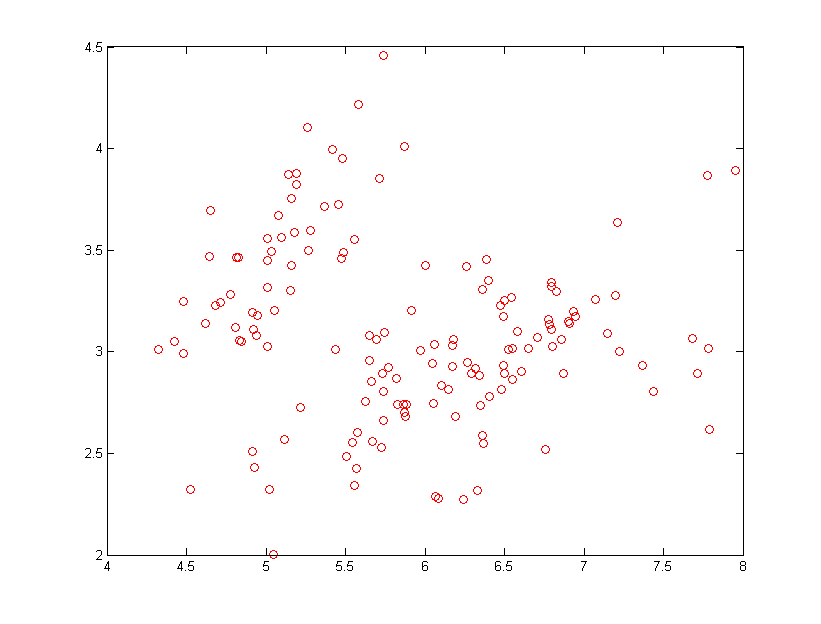
\includegraphics[width=6 in]{prob1PartA.png}
\caption{Raw Iris Data}
\end{figure}

\newpage

\subsection*{Part b}

I tried a few different initializations. I tried the 3 different ones available in the kmeans function as well as my own initialization points. For $k=5$, I arranged 5 points in an X-shape in the $x_1,x_2$ space. For $k=20$, I did two different initial arrangements: a $4x5$ grid and a $5x4$ grid in the $x_1,x_2$ space. For $k=5$ the lowest score came from my initialization. For $k=20$ the lowest score also came from my initialization, specifically the $5x4$ initialization, although the $4x5$ grid had nearly the same score. \\
\\
Here is the best 5-means clustering I was able to achieve
\begin{figure}[h]
\centering
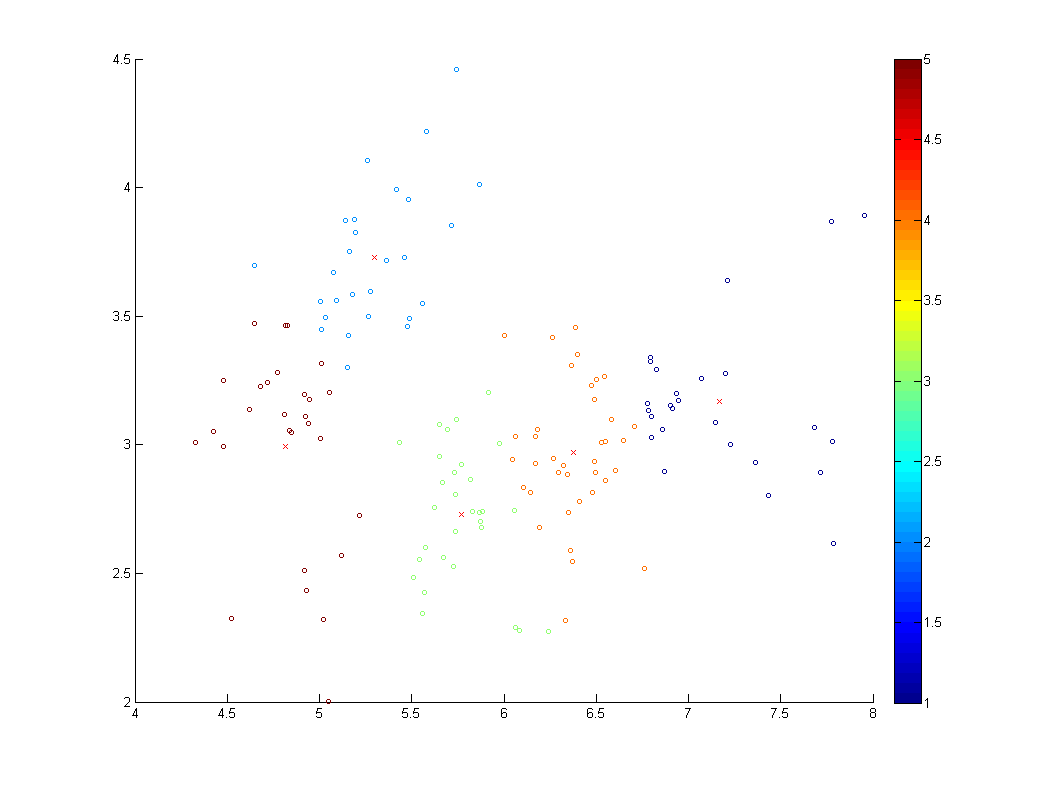
\includegraphics[width=6 in]{prob1PartB_1.png}
\caption{$k=5$ clustering with x marks for cluster centers}
\end{figure}

\newpage

Here is the best 20-means clustering I was able to achieve.
\begin{figure}[h]
\centering
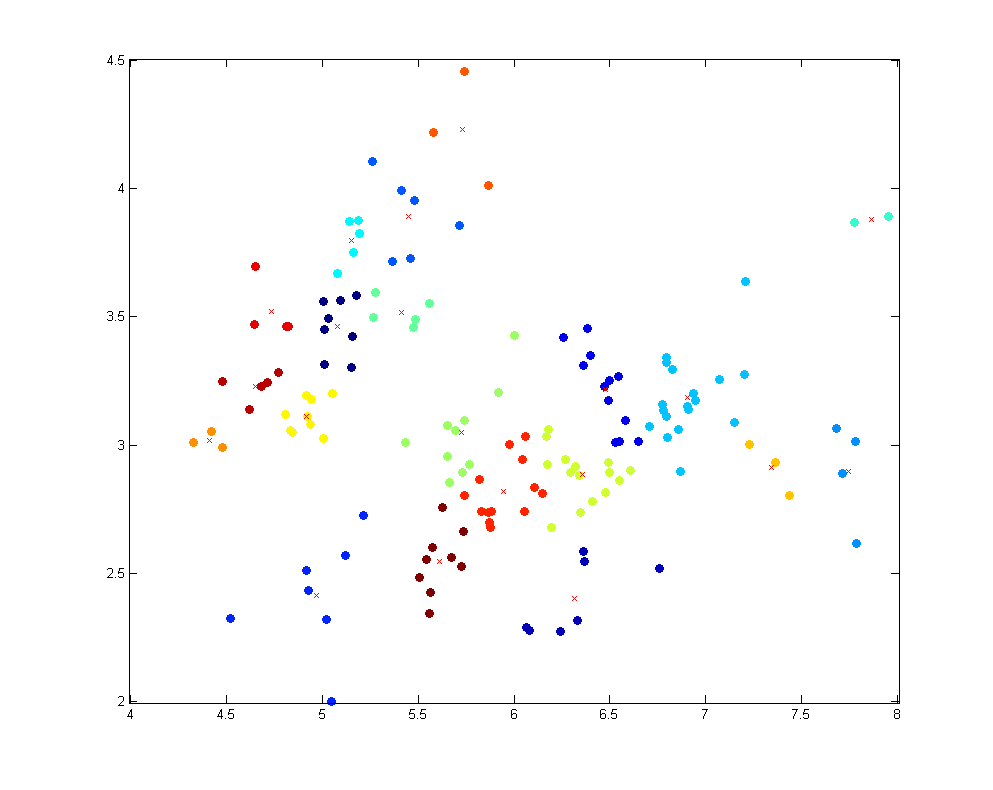
\includegraphics[width=6 in]{prob1PartB_2.png}
\caption{$k=20$ clustering with x marks for cluster centers}
\end{figure}

\newpage

Here is the code for Part A and B.
\lstinputlisting[firstline=1, lastline=93]{prob1.m}

\newpage

\subsection*{Part c}

Here are the plots of agglomerative clustering with 5 clusters.  
\begin{figure}[h]
\centering
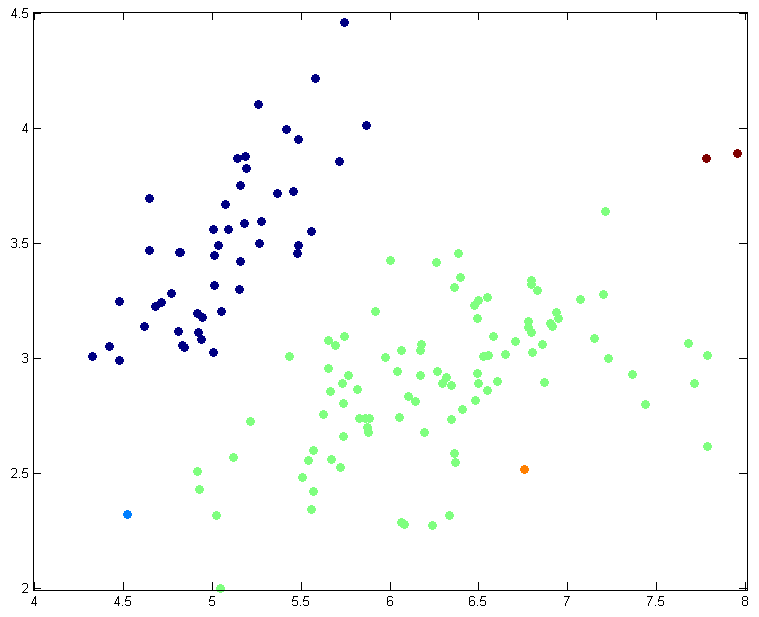
\includegraphics[width=6 in]{prob1PartC_1.png}
\caption{Agglomerative clustering with 5 clusters, single linkage}
\end{figure}

\begin{figure}[h]
\centering
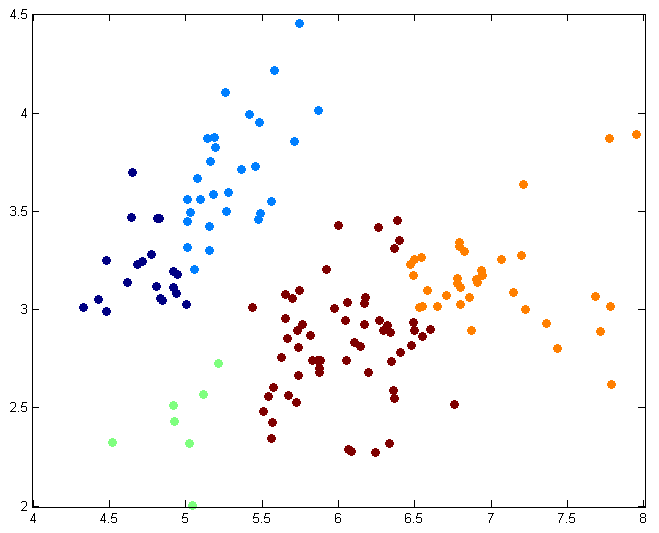
\includegraphics[width=6 in]{prob1PartC_2.png}
\caption{Agglomerative clustering with 5 clusters, complete linkage}
\end{figure}

Here are the plots of agglomerative clustering with 20 clusters.  
\begin{figure}[h]
\centering
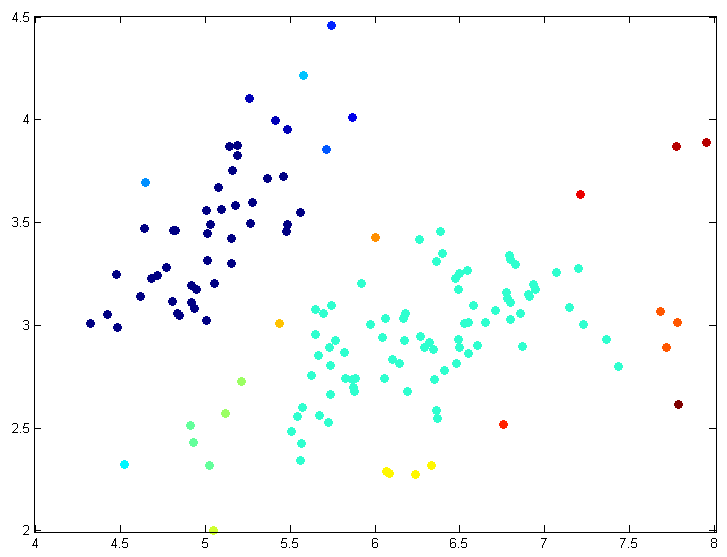
\includegraphics[width=6 in]{prob1PartC_3.png}
\caption{Agglomerative clustering with 20 clusters, single linkage}
\end{figure}

\begin{figure}[h]
\centering
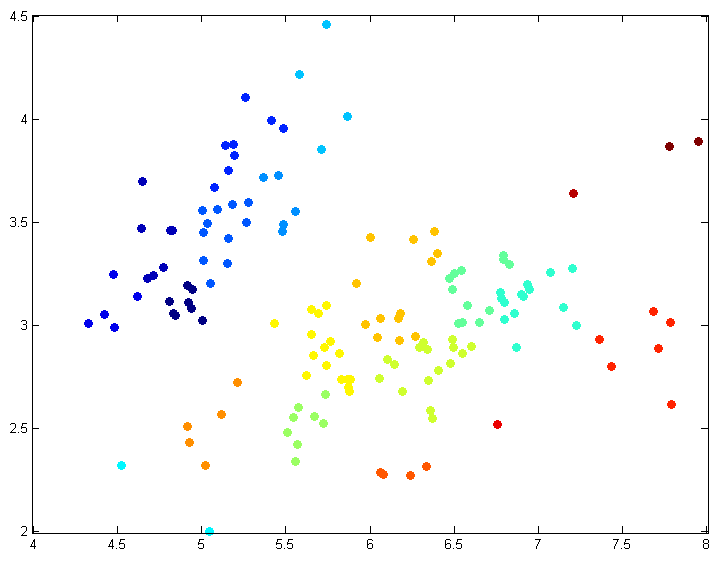
\includegraphics[width=6 in]{prob1PartC_4.png}
\caption{Agglomerative clustering with 20 clusters, complete linkage}
\end{figure}

As can be observed, single linkage tries to group the points into as few clusters as possible whereas complete linkage spreads out the clustering. The results for complete linkage look quite similar to k-Means. 


\end{document}
